\documentclass[dvipsnames,10pt]{article}
\usepackage{graphicx,float}
\usepackage{amsmath, amsfonts, amsthm, amssymb}
\usepackage{braket, nicefrac}
\usepackage{hyperref,mathtools}
\usepackage{tikz}
\usepackage{tikz-cd}
\usepackage{theoremref}
\usepackage[a4paper, total={5.5in, 9.1in}]{geometry}
\usepackage{setspace}
\usepackage{xcolor}
\usepackage{tgpagella}


\newtheorem{theorem}{Theorem}[section]
\newtheorem{lemma}[theorem]{Lemma}
\newtheorem{proposition}[theorem]{Proposition}
\newtheorem{cor}[theorem]{Corollary}
\newtheorem{defi}[theorem]{Definition}
\newtheorem{construction}[theorem]{Construction}
\title{\Large \textbf{The Betti Numbers of Edge Ideals of Trees and the Regularity Offset}}

\date{}

\begin{document}

\setstretch{1.2}
\maketitle

\section{Background}
\subsection{Graphs and clique complexes}
A simple graph $G$ is the composition of vertex set $V(G)$ and edge set $E(G)$. We use $G^c$ to denote the complement graph of $G$. If $W$ is a subset of $V(G)$, we use $G[W]$ to denote the induced subgraph on $W$.

For a simple graph $G$ whose vertex set is $[n]$, one can identify it with
a square-free quadratic ideal $I_G$ over a field $k$ via $I_G=(x_ix_j | ij\in E(G))$. We call $I_G$ the edge ideal of $G$.

\begin{defi}
    Given a graph $G$, where $V(G)=\{x_1,x_2,\cdots,x_n\}$, the clique complex of $G$, denoted by $\Delta G$, is a simplicial complex that consists of $t$-simplicies $(x_{i_1},x_{i_2},\cdots ,x_{i_t})$ whenever $G[\{x_{i_1},x_{i_2},\cdots ,x_{i_t}\}]$ is a complete graph of $t$ vertices.
\end{defi}

One can observe that the edge ideal $I_G$ is the Stanley-Reisner ideal of $\Delta G^c$. Hence, we have a one-to-one correspondence between the family of simple graphs and the family of clique complexes. Moreover, homology of simplicial complexes $\Delta G^c$ can give Betti numbers of $I_G$ via Hochster's formula.

\begin{theorem}\thlabel{hochster}[Hochster's formula]
    Let $I_G$ be the edge ideal of a graph $G$. Then for $i\geq 0$ and square-free degree $\mathbf{b}$,
    \begin{equation*}
        \beta_{i,\mathbf{b}}(I_G)=dim_k(\widetilde{H}_{|\mathbf{b}|-i-2}\left(\Delta G^c[supp(\mathbf{b})], k\right)),
    \end{equation*}
    and $\beta_{i,\mathbf{b}}(I_G)=0$ if $\bf{b}$ is not square-free. If we forget the multigrading, then for $j\geq0$,
    \begin{equation*}
        \beta_{i,i+j}(I_G)=\sum_{|W|=i+j}dim_k(\widetilde{H}_{j-2}\left(\Delta G^c[W], k\right)),
    \end{equation*}
    where $W$ runs over all the subsets of $V(G)$ of size $i+j$.
\end{theorem}
More detailed information on Hochster's formula can be found in \cite{stanley1996combinatorics} and \cite{francisco2014survey}. We now give the definition of Castelnuovo-Mumford regularity of an edge-ideal $I_G$.
\begin{defi}[Castelnuovo-Mumford regularity]\thlabel{regdef}
    We use $reg(I_G)$ (or $reg(G)$ in short) to denote the Castelnuovo-Mumford regularity of $I_G$. 
    \begin{equation*}
    reg(I_G)=max\{j|\beta_{i,i+j}(I_G)\neq0\}.    
    \end{equation*}
\end{defi}

To make the following paper more readable, for a subgraph $S\subset G$, we say the subgraph $S$ contribute to the regularity if the multigraded betti number $\beta_{|\mathbf{s}|-reg(G),\mathbf{s}}\neq 0$, where $\mathbf{s}$ is a grading that is all zero but only $1$s on the variables that are corresponding to the vertex set $V(S)$.

By Hochster's formula, the key part of finding the regularity of an edge ideal is to find the largest number $j$, such that the $(j-2)$-nd homology group of a certain size induced subcomplex of $\Delta G^c$ is non-trivial. 

\subsection{The lcm-lattice}

The lcm-lattice, introduced in \cite{welker1999lcm}, is a convenient way to compute the betti numbers and analyze the minimal free resolution of edge ideals. 

\begin{defi}[\cite{welker1999lcm}, Page 2]
    Let $S=k[x_0,\cdots,x_n]$ be the polynomial ring over a field $k$ and $I=(m_1,\cdots, m_d)$ a monomial ideal with its minimal generators. Its \textbf{lcm-lattice} $L_I$ is the lattice with elements labeled by the least common multiples of $m_1,... ,m_d$ ordered by divisibility, including $1$, which is regarded as the lcm of the empty set.
\end{defi}

If follows immediately that the atoms of $L_I$ are precisely $\{m_1,\cdots,m_d\}$.\\

The relabeling construction from \cite{welker1999lcm} captures the adding variables construction discussed in the previous section.

\begin{construction}
    
\end{construction}
\vspace{-4pt}

Let $I$ and $J$ be monomial ideals in $S=k[x_0,\cdots,x_n]$, and $f:L_I\to L_J$ a map which is a bijection on atoms and preserves joins. Let $\mathbf{P}$ be a bounded chain complex of free modules with homogeneous differentials $\partial^\mathbf{P}$ such that every generator of every free module $\mathbf{P}_n$ has multidegree in $L_I$. The chain complex $f(\mathbf{P})$ is constructed as follows:

Let $\mathbf{P}_n=\bigoplus_{i=1}^{d} S[-\mathbf{a}_i]^{k_i}$, then $f(\mathbf{P})_n=\bigoplus_{i=1}^{d} S[-f(\mathbf{a}_i)]^{k_i}$, where we also consider $f$ as a map $\mathbb{N}^{n+1}\to \mathbb{N}^{n+1}$ between multidegrees.

The differential $\partial^\mathbf{P}_n$ is homogeneous, and thus is a matrix of monomials. Suppose that its $(i,j)$-th entry $c \mathbf{x}^\mathbf{t}$ is nonzero, with $c\in k$. Suppose the $i$-th summand of $\mathbf{P}_{n-1}$ has generator in degree $\mathbf{a}$, and the $j$-th summand of $\mathbf{P}_n$ has generator in degree $\mathbf{b}$, then homogeneity implies $\mathbf{t} = \mathbf{b} - \mathbf{a}$. The differential $\partial^{f(\mathbf{P})}_n$ is the matrix having $(i,j)$-th entry $c \mathbf{x}^{f(\mathbf{b}) - f(\mathbf{a})}$. This makes it the unique homogeneous differential of $f(\mathbf{P})$ having the same $k$-coefficients in every entry as $\partial^\mathbf{P}_n$.\\

The following theorem from \cite{welker1999lcm} states that ideals with isomorphic lcm-lattice have similar minimal free resolutions.

\begin{theorem}[\cite{welker1999lcm}, Theorem 3.3]\thlabel{relabel}
    Let $I$ and $J$ be monomial ideals. Suppose that $f:L_I\to L_J$ is a bijection of the underlying sets and preserves joins. Let $\mathbf{F}$ be the minimal free resolution of $S/I$, then $f(\mathbf{F})$ is the minimal free resolution of $S/J$.
\end{theorem}

\section{Edge Ideals of Trees}

Trees are a type of very simple graphs whose Betti numbers are relatively simple to compute. In this section, we present a new proof to a leaf deletion theorem in \cite{bouchat}, and use it to compute the Betti numbers of forests.

\subsection{Full graphs and a leaf deletion theorem}

By Hochster's formula (\thref{hochster}), the nonzero Betti numbers of a graph can appear only in square-free multidegrees. The largest such multidegree is $\mathbf{1}=(1,\cdots,1)$, and we make the following definition.
\begin{defi}\thlabel{fulldef}
    A \textbf{full graph} is a graph $G$ such that for some $i$ we have $\beta_{i,\mathbf{1}}(I_G)\neq 0$. A \textbf{full subgraph} of a graph $G$ is an induced subgraph $H$ that is itself a full graph.
\end{defi}
We will see later (\thref{fullnameorigin}) that a tree is full if and only if all vertices contribute to its regularity, hence the name `full'.

We now turn to a leaf deletion theorem, implicitly mentioned in \cite{bouchat}, that lies at the core of the computation of tree Betti numbers. We first present an auxiliary lemma (\cite{bouchat}, Theorem 2.1.1) and a detailed proof different from the original proof in \cite{bouchat}.

\begin{lemma}[Mapping cone lemma]\thlabel{mpclemma}
    Let $G$ be a simple graph and $V(G) = \{x_1,\cdots,x_n\}$, with $x_n$ a leaf and $x_{n-1}$ its neighbor. Let $S=k[x_1,\cdots,x_n]$ and
    \begin{align*}
        J&=(x_ix_j\mid \{x_i,x_j\}\in E(G),\,x_ix_j\neq x_{n-1}x_n),\\
        -\mathbf{2} &= (0,\cdots,0,-1,-1),
    \end{align*}
    then there is a short exact sequence
    \begin{equation}
        \begin{tikzcd}
            0 \arrow[r] & S/(J:x_{n-1}x_n)[-\mathbf{2}] \arrow[rr, "{x_{n-1}x_n}"] & & S/J \arrow[r] & S/I_G \arrow[r] & 0.
        \end{tikzcd}
    \end{equation}
    Moreover, let $\mathbf{E}, \mathbf{F}, \mathbf{G}$ be the minimal free resolutions of the three modules in (1), from left to right respectively, then the induced short exact sequence of chain complexes
    \begin{equation*}
        \begin{tikzcd}
            0 \arrow[r] & \mathbf{E} \arrow[r, "\phi"] & \mathbf{F} \arrow[r] & \mathbf{G} \arrow[r] & 0
        \end{tikzcd}
    \end{equation*}
    presents $\mathbf{G}$ as the mapping cone of $\phi$.
\end{lemma}

\begin{proof}
    It is clear that (1) is an exact sequence. For the second statement, as minimal free resolutions are unique up to isomorphism, it suffices to prove that the mapping cone $\mathbf{H}=C(\phi)$ is a minimal free resolution of $S/I_G$. It is a complex of free modules by definition, and by the long exact sequence of homology it is a resolution of $S/I_G$. To prove it is minimal, we need to prove that there are no non-zero constants in the (matrices of the) differentials of $\mathbf{H}$. As $\mathbf{E}$ and $\mathbf{F}$ are both minimal, there are no nonzero constants in their differentials. By the structure of the differentials of the mapping cone, it suffices to show that there are no nonzero constants in every $\phi_i$.
    
    Consider the construction of the induced chain map $\phi$.
    \begin{equation*}
        \begin{tikzcd}
            \cdots \arrow[r] & \mathbf{E}_{t+1} \arrow[r, "{d_{t+1}^\mathbf{E}}"] \arrow[d,"{\phi_{t+1}}"] & \mathbf{E}_t \arrow[r, "{d_{t}^\mathbf{E}}"]\arrow[d,"{\phi_{t}}"] & \mathbf{E}_{t-1}\arrow[r, "{d_{t-1}^\mathbf{E}}"]\arrow[d,"{\phi_{t-1}}"]  & \cdots \\
            \cdots \arrow[r]  & \mathbf{F}_{t+1}\arrow[r, "{d_{t+1}^\mathbf{F}}"]  & \mathbf{F}_t \arrow[r, "{d_{t}^\mathbf{F}}"] & \mathbf{F}_{t-1}\arrow[r, "{d_{t-1}^\mathbf{F}}"]  & \cdots
        \end{tikzcd}
    \end{equation*}
    Set $\mathbf{E}_{-1}=S/(J:x_{n-1}x_n)$ and $\mathbf{F}_{-1}=S/J$ and $\phi_{-1}=x_{n-1}x_n$, then $\mathbf{E}$ and $\mathbf{F}$ both become exact complexes. The inductive construction of $\phi$ is as follows. Having constructed $\phi_t$, we have $d_t^\mathbf{F}\,\phi_t\,d_{t+1}^\mathbf{E}=\phi_{t-1}\,d_{t}^\mathbf{E}\,d_{t+1}^\mathbf{E}=0$, so $\mathrm{im}(\phi_t\,d_{t+1}^\mathbf{E})\subset \ker d_t^\mathbf{F}=\mathrm{im}\:d_{t+1}^\mathbf{F}$. For every generator $e_i$ of $\mathbf{E}_{t+1}$, pick a $f_i\in \mathbf{F}_{t+1}$ such that $d_{t+1}(f_i)=\phi_t(d_{t+1}(e_i))$, and this selection defines the map $\phi_{t+1}$.
    
    We now prove by induction that the image of every $\phi_t$ lies in $x_n\mathbf{F}_t$, which proves the lemma. Suppose that this is true for $\phi_t$, then for every generator $e_i$ of $\mathbf{F}_{t+1}$ we have $\phi_t(d_{t+1}(e_i))=x_n\epsilon_i$ for some $\epsilon_i\in \mathbf{F}_t$. Now $x_n\epsilon_i\in \ker d_{t}^\mathbf{F}$ implies that $x_nd_t^{\mathbf{F}}(\epsilon_i)=0$ in $\mathbf{F}_{t-1}$. When $t\geqslant 1$, $\mathbf{F}_{t-1}$ is a free module which has no torsion, so $d_t^{\mathbf{F}}(\epsilon_i)=0$. Therefore $\epsilon_i\in \ker d_{t}^\mathbf{F}=\mathrm{im}\: d_{t+1}^\mathbf{F}$. Therefore there exists $f_i\in \mathbf{F}_{t+1}$ such that $d_{t+1}(f_i)=\epsilon_i$. The map $\phi_{t+1}$ can be taken to send $e_i$ to $x_nf_i$.

    The above inductive step only holds for $t\geqslant 1$, so we still have to prove the base cases $t=-1,0,1$. The cases $t=-1$ and $0$ are obvious, as $\phi_{-1}$ and $\phi_0$ are both multiplication by $x_{n-1}x_n$. For the final case $\phi_1$, we can still use the inductive step with $t=0$, because although $\mathbf{F}_{-1}=S/J$ is not torsion-free, $x_n\xi=0$ still implies $\xi=0$ for $\xi\in S/J$.
\end{proof}

By Hochster's formula, the non-zero Betti numbers of graphs only appear in square-free multidegrees. square-free multidegrees are in one-to-one correspondence with subsets of the vertex set, so we introduce the following notation. For a graph $G$ with $V(G)=\{x_1,\cdots,x_n\}$ and a subset $H\subset V(G)$, write $\beta_i(G,H)$ for the betti number $\beta_{i,\mathbf{a}}(k[V(G)]/I_G)$, where $a_i=1$ when $x_i\in H$ and $a_i=0$ when $x_i\notin H$. We abbreviate $\beta_i(G,V(G))$ as $\beta_i(G)$, so full graphs are graphs with $\beta_i(G)=1$ for some $i$.

\begin{theorem}[Leaf deletion theorem]\thlabel{deletion}
    Let $G$ be a graph with $V(G)=\{x_1,\cdots,x_n\}$ and $H\subset V(G)$. Suppose $x_n$ is a leaf of $G$ and $x_{n-1}$ its neighbor. Then
    \begin{equation*}
        \beta_i(G,H) = \left\{
            \begin{aligned}
                &\beta_i(G\setminus x_n,H), &x_n\notin H,\\
                &\beta_{i-\#(N(x_{n-1})\cap H)}(G_{(n)},H\cap G_{(n)}), &x_{n-1}\in H,x_n\in H,\\
                &0, &x_{n-1}\notin H,x_n\in H.
            \end{aligned}
        \right.
    \end{equation*}
    The set $N(x_{n-1})$ is the open neighborhood of $x_{n-1}$ in $G$.\\
    The graph $G_{(n)}$ is the induced subgraph of $G$ on $\{\,x_i\mid \{x_i,x_{n-1}\}\notin E(G),\;i\neq n-1\,\}$. That is, it is the induced subgraph on all vertices not adjacent to $x_{n-1}$ and not equal to it.\\
    To deal with the case where $G_{(n)}=\varnothing$ is the empty graph, we define $\beta_i(\varnothing,\varnothing)=1$ when $i=0$ and $\beta_i(\varnothing,\varnothing)=0$ otherwise.
\end{theorem}

\begin{proof}
    Let $\mathbf{a}$ be the indicator multidegree of $H$, and $S=k[V(G)]$. By \thref{mpclemma} we have $\mathbf{G}_i=\mathbf{F}_i\oplus \mathbf{E}_{i-1}$. Therefore
    \begin{align}
        \beta_i(G,H) = \beta_{i,\mathbf{a}}(S/I_G) &= \beta_{i,\mathbf{a}}(S/J) + \beta_{i-1,\mathbf{a}}(S/(J:x_{n-1}x_n)[-\mathbf{2}])\\
        &= \beta_{i,\mathbf{a}}(S/J) + \beta_{i-1,\mathbf{a}-\mathbf{2}}(S/(J:x_{n-1}x_n)).
    \end{align}
    Observe that $J$ is an ideal contained in the subring $k[x_1,\cdots,x_{n-1}]\subset S$, therefore its minimal free resolution considered on $S$ is the same as its minimal free resolution considered on $k[x_1,\cdots,x_{n-1}]$, just with a different base ring. Using the notation of \thref{mpclemma}, no generator of $\mathbf{F}_i$ has a multidegree $\mathbf{a}$ with $a_n\neq 0$. This means that
    \begin{equation}
        \beta_{i,\mathbf{a}}(S/J) = \left\{
            \begin{aligned}
                &\beta_{i,\,(a_1,\cdots,a_{n-1})}(k[x_1,\cdots,x_{n-1}]/I_J)=\beta_i(G\setminus x_n,H), &a_n=0,\\
                &0, &a_n=1.
            \end{aligned}
        \right.
    \end{equation}

    On the other hand, we have
    \begin{equation*}
        (J:x_{n-1}x_n) = (J:x_{n-1}) = I_{G_{(n)}} + (x_i\mid x_i\in N(x_{n-1})\setminus x_n).
    \end{equation*}
    Write $K=(x_i\mid x_i\in N(x_{n-1})\setminus x_n)$, then $I_{G_{(n)}}$ and $K$ have completely disjoint generators. By the technical lemma presented after this proof (\thref{tensor}), we have
    \begin{align*}
        &\beta_{i-1,\mathbf{a}-\mathbf{2}}(S/(J:x_{n-1}x_n)) \\
        &= \sum_{s+t=i-1}\beta_{s,(\mathbf{a}-\mathbf{2})[V(G_{(n)})]}(k[V(G_{(n)})]/I_{G_{(n)}})\,\cdot\,\beta_{t,(\mathbf{a}-\mathbf{2})[N(x_{n-1})\setminus x_n]}(k[N(x_{n-1})\setminus x_n]/K).
    \end{align*}
    Now $K$ is generated by single variables, so its minimal free resolution is the Kozsul complex on these variables. Therefore $\beta_{t,(\mathbf{a}-\mathbf{2})[N(x_{n-1})\setminus x_n]}(k[N(x_{n-1})\setminus x_n]/K)\neq 0$ if and only if $\mathbf{a}-\mathbf{2}\geqslant \mathbf{0}$ and $t$ is the number of $1$'s in $\mathbf{a}-\mathbf{2}$. This is equivalent to $a_{n-1}=a_n=1$ and $t$ equal to the number of $a_i$'s such that $a_i=1$ and $1\leqslant i<n-1$. In this case $\beta_{t,(\mathbf{a}-\mathbf{2})[N(x_{n-1})\setminus x_n]}(k[N(x_{n-1})\setminus x_n]/K)=1$ and $s=i-1-t=i-\#(N(x_{n-1})\cap H)$, so
    \begin{equation*}
        \beta_{s,(\mathbf{a}-\mathbf{2})[V(G_{(n)})]}(k[V(G_{(n)})]/I_{G_{(n)}}) = \beta_{i-\#(N(x_{n-1})\cap H)}(G_{(n)},H\cap G_{(n)}).
    \end{equation*}
    Therefore
    \begin{equation}
        \beta_{i-1,\mathbf{a}-\mathbf{2}}(S/(J:x_{n-1}x_n)) = \left\{
            \begin{aligned}
                &\beta_{i-\#(N(x_{n-1})\cap H)}(G_{(n)},H\cap G_{(n)}), &a_{n-1}=a_n=1,\\
                &0, &\mathrm{otherwise}.
            \end{aligned}
        \right.
    \end{equation}
    The above reasoning assumed $N(x_{n-1})\setminus x_n\neq\varnothing$. If $N(x_{n-1})\setminus x_n=\varnothing$ then $(J:x_{n-1}x_n)=I_{G_{(n)}}$ and $\#(N(x_{n-1})\cap H)=1$, and so formula (5) follows directly.

    Now the theorem follows from the formulas (3)(4)(5) when $G_{(n)}\neq \varnothing$. When $G_{(n)}= \varnothing$, $G$ is a star with center $x_{n-1}$, and we assume $x_{n-1},x_n\in H$ because this is always true when $G_{(n)}$ appears in the theorem. For convenience, relabel the vertices of $G$ as $\{y_0,y_1,\cdots,y_t\}$ with the center being $y_0$ and such that $y_0,y_1\in H$, so $I_G=(y_0y_1,\cdots,y_0y_t)$. Let $S=k[y_0,\cdots,y_t]$ then the minimal free resolution of $S/I_G$ is almost the Koszul complex on $\{y_1,\cdots,y_t\}$. The only difference is the differential in degree $0$: instead of $(y_1,\cdots,y_t)$ it is $(y_0y_1,\cdots,y_0y_t)$. We are assuming $y_0,y_1\in H$, and in this case the Betti number $\beta_i(G,H)=1$ if and only if $i=\#(H\cap \{y_1,\cdots,y_t\})=\#(N(y_0)\cap H)$. Therefore the theorem holds precisely when $\beta_i(\varnothing,\varnothing)$ is defined the way it is defined in the statement of the theorem.
\end{proof}

The above proof used the following lemma.

\begin{lemma}\thlabel{tensor}
    Let $S=k[x_1,\cdots,x_m]$ and $T=k[y_1,\cdots,y_n]$, with $I\subset S$ and $J\subset T$ monomial ideals. Let $R=k[x_1,\cdots,x_m,y_1,\cdots,y_n]$ and $I',J'$ ideals of $R$ with the same generators as $I$ and $J$ respectively. Let $\mathbf{a}\in\mathbb{N}^m$ and $\mathbf{b}\in\mathbb{N}^n$. Then
    \begin{equation*}
        \beta_{i,(\mathbf{a},\mathbf{b})}^R(R/(I'+J')) = \sum_{i+j=t}\beta_{i,\mathbf{a}}^S(S/I)\beta_{j,\mathbf{b}}^T(T/J),
    \end{equation*}
    where $\beta_t^R$ denotes that the free resolution uses free $R$-modules.
\end{lemma}

\begin{proof}
    It is clear that
    \begin{align*}
        \beta_{i,\mathbf{a}}^S(S/I)&=\beta_{i,(\mathbf{a},0)}^R(R/I'),\\
        \beta_{j,\mathbf{b}}^T(T/J)&=\beta_{j,(0,\mathbf{b})}^R(R/J').
    \end{align*}
    Therefore we only need to prove
    \begin{equation*}
        \beta_{i,(\mathbf{a},\mathbf{b})}^R(R/(I'+J')) = \sum_{i+j=t}\beta_{i,(\mathbf{a},0)}^R(R/I')\beta_{j,(0,\mathbf{b})}^R(R/J').
    \end{equation*}
    Let $\mathbf{F}$ and $\mathbf{G}$ be the minimal free resolutions of $R/I'$ and $R/J'$ respectively, then the generators in $\mathbf{F}_i$ can only have multidegrees $(\mathbf{a},0)$ and the generators in $\mathbf{G}_j$ can only have multidegrees $(0,\mathbf{b})$. Consider the tensor product complex $\mathbf{H}=\mathbf{F}\otimes_R \mathbf{G}$. The tensor product of a generator of degree $(\mathbf{a},0)$ and a generator of degree $(0,\mathbf{b})$ is a generator in $\mathbf{H}_{i+j}$ of degree $(\mathbf{a},\mathbf{b})$. If $\mathbf{H}$ is the minimal free resolution of $R/(I'+J')$ then the above formula follows immediately.

    The matrix of $d_t^\mathbf{H}$ is consists of the matrix tensor products $d_i^\mathbf{F}\otimes d_j^\mathbf{G}$ for $i+j=t$. Now $\mathbf{F}$ and $\mathbf{G}$ being minimal implies that $d_i^\mathbf{F}$ and $d_j^\mathbf{G}$ has no nonzero constants, so $d_i^\mathbf{F}\otimes d_j^\mathbf{G}$ has no nonzero constants, and so $\mathbf{H}$ is minimal if it is a resolution.

    To prove $\mathbf{H}$ is a resolution, we use the spectral sequence $\{E_{i,j}^d\}$ of the total complex $\{\mathbf{F}_i\otimes \mathbf{G}_j\}_{i,j}$. The $1$st page $\{E^1_{i,j}\}$ consists of the homology of the rows $\mathbf{F}_{\ast}\otimes \mathbf{G}_j$ of the double complex. As each $\mathbf{G}_j$ is free so flat, we have $E^1_{i,j}=H_i(\mathbf{F})\otimes \mathbf{G}_j$, so $E^1_{i,j}=0$ when $i\neq 0$ and $E^1_{0,j}=(R/I')\otimes \mathbf{G}_j$. The differentials $d^1_{0,j}=(R/I')\otimes d^\mathbf{G}_j$. Therefore the $2$nd page is $E^2_{0,j}=\mathrm{Tor}_j(R/I',R/J')$ and $E^2_{i,j}=0$ when $i\neq 0$. The differentials $d^2_{i,j}=0$, so $E^\infty_{i,j}=E^2_{i,j}$. Therefore the homology $H_t(\mathbf{F}\otimes \mathbf{G})\cong\mathrm{Tor}_t(R/I',R/J')$. As $I'$ and $J'$ are monomial ideals whose generators are formed by two disjoint sets of variables, a simple computation shows that $\mathrm{Tor}_t(R/I',R/J')=0$ when $t>0$, so $\mathbf{H}$ is indeed a resolution of $\mathrm{Tor}_0(R/I',R/J')=R/I'\otimes R/J'\cong R/(I'+J')$.
\end{proof}

\subsection{Computing Betti numbers}

Now we turn to the computation of $\beta_i(G,H)$ for forests. \thref{deletion} provides us with a powerful tool, letting us delete leaves and reduce a forest inductively into trivial forms. We first take a look at the trivial case.

\begin{proposition}\thlabel{edgeless}
    Let $G$ be an edgeless graph with $V(G)=\{x_1,\cdots,x_t\}$ ($t\geqslant 0$) and $H\subset V(G)$, then $\beta_i(G,H)=1$ when $H=\varnothing$ and $i=0$, and $\beta_i(G,H)=0$ otherwise.
\end{proposition}

\begin{proof}
    The ideal $I_G=0$, and its ambient ring is $S=k[x_1,\cdots,x_t]$. Its minimal free resolution is $0\to S\to 0$, so its only nonzero Betti number is $1$, lying in the multidegree $\mathbf{0}$ and homological degree $i=0$.
\end{proof}

\begin{theorem}\thlabel{subtree}
    Let $T$ be a forest and $H\subset V(T)$, then $\beta_i(T,H)$ can only be $0$ or $1$, and we have
    \begin{equation*}
        \beta_i(T,H)=\beta_i(T[H],H).
    \end{equation*}
    Therefore, $\beta_i(T,H)=1$ only when $T[H]$ is a full graph.
\end{theorem}

\begin{proof}
    We provide an algorithmic procedure of deleting parts of the forest $T$ until only an edgeless graph remains. Initialize the $6$-tuple as:
    \begin{equation*}
        (i_0,A_0,B_0,j_0,C_0,D_0)\coloneq (i,T,H,i,T[H],H).
    \end{equation*}
    From $(i_t,A_t,B_t,j_t,C_t,D_t)$, pick a leaf $x_n$ and its neighbor $x_{n-1}$ in the graph $A_t$ and construct $(i_{t+1},A_{t+1},B_{t+1},j_{t+1},C_{t+1},D_{t+1})$ as follows.\\
    \textbf{Case 1:} $x_n\notin B_t$. Set
    \begin{align*}
        i_{t+1}&\coloneq i_t,\\
        A_{t+1}&\coloneq A_t\setminus x_n,\\
        B_{t+1}&\coloneq B_t,\\
        j_{t+1}&\coloneq j_t,\\
        C_{t+1}&\coloneq C_t,\\
        D_{t+1}&\coloneq D_t.
    \end{align*}
    \textbf{Case 2:} $x_{n-1}\in B_t,x_n\in B_t$. Set
    \begin{align*}
        i_{t+1}&\coloneq i_t-\#(N_{A_t}(x_{n-1})\cap B_t),\\
        A_{t+1}&\coloneq A_t[V(A_t)\setminus N_{A_t}(x_{n-1})\cup\{x_{n-1}\}],\\
        B_{t+1}&\coloneq B_t\cap V(A_{t+1}),\\
        j_{t+1}&\coloneq j_t-\#(N_{C_t}(x_{n-1})\cap D_t),\\
        C_{t+1}&\coloneq C_t[V(C_t)\setminus N_{C_t}(x_{n-1})\cup\{x_{n-1}\}],\\
        D_{t+1}&\coloneq D_t\cap V(C_{t+1}).
    \end{align*}
    \textbf{Case 3:} $x_{n-1}\notin B_t,x_n\in B_t$. Terminate.\\
    \textbf{Case 4:} $A_t$ is an edgeless graph. Terminate.

    There are a few things to prove. First, it is clear from \thref{deletion} that $\beta_{i_t}(A_t,B_t)=\beta_{i_{t+1}}(A_{t+1},B_{t+1})$ and $\beta_{j_t}(C_t,D_t)=\beta_{j_{t+1}}(C_{t+1},D_{t+1})$. Therefore $\beta_{i_t}(A_t,B_t)=\beta_{i}(T,H)$ and $\beta_{j_t}(C_t,D_t)=\beta_{i}(T[H],H)$. Second, we have the following relations.
    \begin{align*}
        C_t&=A_t[B_t],\\
        D_t&=B_t,\\
        j_t&=i_t.
    \end{align*}
    For Case 1 they are obvious. For Case 2, we prove them inductively on $t$. Suppose that they hold for $t$, then:\\
    (1) $C_{t+1}$ consists of the vertices in $C_t=A_t[B_t]$ that are not adjacent to $x_{n-1}$ and not equal to $x_{n-1}$, and $A_{t+1}$ consists of the vertices in $A_t$ that are not adjacent to $x_{n-1}$ and not equal to $x_{n-1}$. Therefore, the vertices of $C_{t+1}$ are precisely the vertices of $A_{t+1}$ that lie in $B_t$, so $C_{t+1}=A_{t+1}[B_t\cap V(A_{t+1})]=A_{t+1}[B_{t+1}]$.\\
    (2) $D_{t+1}=D_t\cap V(C_{t+1})=B_t\cap V(A_{t+1}[B_{t+1}])=B_{t+1}$.\\
    (3) $V(C_t)=V(A_t[B_t])=B_t=D_t$, so $N_{C_t}(x_{n-1})\cap D_t=N_{C_t}(x_{n-1})=N_{A_t[B_t]}(x_{n-1})=N_{A_t}(x_{n-1})\cap B_t$. Therefore $j_t=i_t$ implies $j_{t+1}=i_{t+1}$.\\
    These results show that
    \begin{align*}
        \beta_i(T,H)&=\beta_{i_t}(A_t,B_t),\\
        \beta_i(T[H],H)&=\beta_{i_t}(A_t[B_t],B_t).
    \end{align*}
    The operations of Case 1 and Case 2 are only valid when both $A_t$ and $C_t$ have at least one edge. If $A_t$ is edgeless then we reach Case 3 which terminates the algorithm. If $C_t$ is edgeless but $A_t$ is not, then $C_t=A_t[B_t]$ is a union of isolated points of $A_t$, and so the connected components that contain edges are disjoint from the vertex set $B_t$, so we can choose a leaf from these components and this will fall into Case 1. This shows that this algorithm can indeed run until it terminates at Case 3 or Case 4.
    
    If the algorithm terminates at Case 3, then $\beta_{i_t}(A_t,B_t)=0$ by \thref{deletion}. The subforest $C_t$ has an isolated point, so $\beta_{i_t}(C_t)=0$. Therefore $\beta_i(T,H)=\beta_i(T[H],H)=0$.

    If the algorithm terminates at Case 4, then $A_t$ is an edgeless graph. By \thref{edgeless}, $\beta_{i_t}(A_t,B_t)=1$ precisely when $i_t=0$ and $B_t=\varnothing$, and this is also precisely when $\beta_{i_t}(A_t[B_t],B_t)=1$. Therefore $\beta_i(T,H)=\beta_i(T[H],H)$.
\end{proof}

\thref{subtree} shows that the nonzero Betti numbers of forests only occur in full subforests. Therefore the problem of computing all Betti numbers of forests is reduced to finding full forests and the right $i$ such that $\beta_i(T,V(T))=1$ when $T$ is full.

\begin{defi}\thlabel{deletiondef}
    Let $T$ be a forest. Define the \textbf{deletion operation} as: Pick a leaf and denote its neighbor by $v$, then delete the closed neighborhood of $v$ from the tree. By deleting a set of vertices, we mean removing all vertices in this set and all edges with at least one endpoint in this set. This deletion operation is always possible when $T$ is not edgeless.
\end{defi}

\begin{theorem}\thlabel{full}
    Let $T$ be a forest, then $T$ is full if and only if $T$ can be reduced to the empty graph using the deletion operation. When $T$ is full, denote by $N$ the number of deletion operations performed to reduce it to the empty graph, then $\beta_i(T,V(T))=1$ precisely when $i=|V(T)|-N$.
\end{theorem}

\begin{proof}
    Similar to the proof of \thref{subtree}, we define the following algorithm. Initialize the $2$-tuple as:
    \begin{equation*}
        (i_0,A_0)\coloneq (i,T).
    \end{equation*}
    From $(i_t,A_t)$, construct $(i_{t+1},A_{t+1})$ as follows.\\
    \textbf{Case 1:} $A_t$ is not edgeless. Pick a leaf $x_n$ and its neighbor $x_{n-1}$ in the graph $A_t$, and set
    \begin{align*}
        i_{t+1}&\coloneq i_t-\#N_{A_t}(x_{n-1}),\\
        A_{t+1}&\coloneq A_t[V(A_t)\setminus N_{A_t}(x_{n-1})\cup\{x_{n-1}\}].
    \end{align*}
    \textbf{Case 2:} $A_t$ is edgeless. Terminate.

    By \thref{deletion} it is clear that $\beta_{i_t}(A_t,V(A_t))$ stays constant throughout the algorithm. The algorithm must terminate as the number of edges in $A_t$ strictly decreases with every step. Let $N$ be the terminating step, then $A_N$ is an edgeless graph. By \thref{edgeless}, $\beta_{i}(T,V(T))=\beta_{i_N}(A_N,V(A_N))=1$ if and only if the terminating edgeless graph is empty and $i_N=0$. In each step, $i_t$ decreases by $\# N(x_{n-1})$, which is the number of vertices deleted minus 1. Therefore, if $A_N$ is empty then $i-i_N=|V(T)|-N$, and $i_N=0$ means $i=|V(T)|-N$.
\end{proof}

\paragraph*{Remark} The choices of the leaf is arbitrary in the algorithm of the above proof, but the result implies that the number of steps does not depend on the choices.

Putting together all the results of this section, we have the following theorem.

\begin{theorem}
    Let $T$ be a forest with $n$ vertices. Let $S=k[x_1,\cdots,x_n]$ and $\mathbf{a}\in\mathbb{N}^n$. Let $H=\mathrm{supp}(\mathbf{a})\subset V(T)$. Then $\beta_{i,\mathbf{a}}(S/I_T)=1$ precisely when all of the following conditions hold, and $\beta_{i,\mathbf{a}}(S/I_T)=0$ otherwise.\\
    \textbf{(1)} $\mathbf{a}$ is square-free.\\
    \textbf{(2)} $T[H]$ is full.\\
    \textbf{(3)} $i=|H|-N$, where $N$ is the number of deletion operations required to reduce $T[H]$ to $\varnothing$.
\end{theorem}

We now provide a faster deletion operation that makes it easier to determine whether a tree is full.

Let $T$ be a tree and $x,y\in V(T)$. There is a unique path between $x$ and $y$, which we denote as $P(x,y)$, both ends inclusive. We denote the length of this path by $d(x,y)$. Now let $x$ be a leaf and define the following \textbf{special neighborhood}:
\begin{equation*}
    \tilde{N}(x) \coloneq \{\,y\in V(T)\mid P(x,y)\text{ does not contain a vertex }z\text{ such that }\deg z \neq 2\text{ and }3\,|\,d(x,z)\,\}.
\end{equation*}

\begin{theorem}\thlabel{fast}
    Let $T$ be a tree and $x$ a leaf, then the subforest
    \begin{equation*}
        T\setminus \tilde{N}(x) = T[V(T)\setminus \tilde{N}(x)]
    \end{equation*}
    can be obtained from $T$ by performing a certain number of deletion operations (\thref{deletiondef}).
\end{theorem}

We now use the previous results to classify full paths and full spiders.

\begin{proposition}
    Let $T_n$ be the path of length $n$, then $T_n$ is full if and only if $3\nmid n$.
\end{proposition}

\begin{proof}
    Let $x,y$ be the two leaves of $T_n$. If $3\,|\,n$ then $\tilde{N}(x)=V(T_n)\setminus \{y\}$, and if $3\nmid n$ then $\tilde{N}(x)=V(T_n)$. The result follows from \thref{fast} and \thref{full}.
\end{proof}

We call a graph with precisely one vertex of degree $>2$ a \textbf{spider}. We call this vertex the center, and call by limbs the paths between the center and a leaf.


\vspace{10pt}
\begin{center}
\tikzset{every picture/.style={line width=0.75pt}} %set default line width to 0.75pt        

\begin{tikzpicture}[x=0.75pt,y=0.75pt,yscale=-1,xscale=1]
%uncomment if require: \path (0,300); %set diagram left start at 0, and has height of 300

%Shape: Circle [id:dp9289362474454589] 
\draw   (99.69,165.31) .. controls (99.69,162.55) and (101.93,160.31) .. (104.69,160.31) .. controls (107.45,160.31) and (109.69,162.55) .. (109.69,165.31) .. controls (109.69,168.07) and (107.45,170.31) .. (104.69,170.31) .. controls (101.93,170.31) and (99.69,168.07) .. (99.69,165.31) -- cycle ;
%Shape: Circle [id:dp5246857754473603] 
\draw   (99.69,105.31) .. controls (99.69,102.55) and (101.93,100.31) .. (104.69,100.31) .. controls (107.45,100.31) and (109.69,102.55) .. (109.69,105.31) .. controls (109.69,108.07) and (107.45,110.31) .. (104.69,110.31) .. controls (101.93,110.31) and (99.69,108.07) .. (99.69,105.31) -- cycle ;
%Shape: Circle [id:dp6671323602377446] 
\draw   (99.69,45.31) .. controls (99.69,42.55) and (101.93,40.31) .. (104.69,40.31) .. controls (107.45,40.31) and (109.69,42.55) .. (109.69,45.31) .. controls (109.69,48.07) and (107.45,50.31) .. (104.69,50.31) .. controls (101.93,50.31) and (99.69,48.07) .. (99.69,45.31) -- cycle ;
%Shape: Circle [id:dp65022849880934] 
\draw   (39.69,165.31) .. controls (39.69,162.55) and (41.93,160.31) .. (44.69,160.31) .. controls (47.45,160.31) and (49.69,162.55) .. (49.69,165.31) .. controls (49.69,168.07) and (47.45,170.31) .. (44.69,170.31) .. controls (41.93,170.31) and (39.69,168.07) .. (39.69,165.31) -- cycle ;
%Shape: Circle [id:dp6418268728639224] 
\draw   (159.69,165.31) .. controls (159.69,162.55) and (161.93,160.31) .. (164.69,160.31) .. controls (167.45,160.31) and (169.69,162.55) .. (169.69,165.31) .. controls (169.69,168.07) and (167.45,170.31) .. (164.69,170.31) .. controls (161.93,170.31) and (159.69,168.07) .. (159.69,165.31) -- cycle ;
%Shape: Circle [id:dp2787063229807829] 
\draw   (219.69,165.31) .. controls (219.69,162.55) and (221.93,160.31) .. (224.69,160.31) .. controls (227.45,160.31) and (229.69,162.55) .. (229.69,165.31) .. controls (229.69,168.07) and (227.45,170.31) .. (224.69,170.31) .. controls (221.93,170.31) and (219.69,168.07) .. (219.69,165.31) -- cycle ;
%Shape: Circle [id:dp7561010118204929] 
\draw   (99.69,225.31) .. controls (99.69,222.55) and (101.93,220.31) .. (104.69,220.31) .. controls (107.45,220.31) and (109.69,222.55) .. (109.69,225.31) .. controls (109.69,228.07) and (107.45,230.31) .. (104.69,230.31) .. controls (101.93,230.31) and (99.69,228.07) .. (99.69,225.31) -- cycle ;
%Shape: Circle [id:dp9372627879078528] 
\draw   (99.69,285.31) .. controls (99.69,282.55) and (101.93,280.31) .. (104.69,280.31) .. controls (107.45,280.31) and (109.69,282.55) .. (109.69,285.31) .. controls (109.69,288.07) and (107.45,290.31) .. (104.69,290.31) .. controls (101.93,290.31) and (99.69,288.07) .. (99.69,285.31) -- cycle ;
%Shape: Circle [id:dp11961602919951786] 
\draw   (280.69,165.31) .. controls (280.69,162.55) and (282.93,160.31) .. (285.69,160.31) .. controls (288.45,160.31) and (290.69,162.55) .. (290.69,165.31) .. controls (290.69,168.07) and (288.45,170.31) .. (285.69,170.31) .. controls (282.93,170.31) and (280.69,168.07) .. (280.69,165.31) -- cycle ;
%Straight Lines [id:da1245642006604587] 
\draw    (104.69,50.31) -- (104.69,100.31) ;
%Straight Lines [id:da4502484852521308] 
\draw    (104.69,110.31) -- (104.69,160.31) ;
%Straight Lines [id:da26939361128521044] 
\draw    (104.69,170.31) -- (104.69,220.31) ;
%Straight Lines [id:da8438010501555864] 
\draw    (104.69,230.31) -- (104.69,280.31) ;
%Straight Lines [id:da011768680116380548] 
\draw    (49.69,165.31) -- (99.69,165.31) ;
%Straight Lines [id:da6006030329211683] 
\draw    (109.69,165.31) -- (159.69,165.31) ;
%Straight Lines [id:da24497375752902406] 
\draw    (169.69,165.31) -- (219.69,165.31) ;
%Straight Lines [id:da057457900131846595] 
\draw    (229.69,165.31) -- (280.69,165.31) ;




\end{tikzpicture}\\
\vspace{6pt}
A spider with limbs of length 1,2,2,3.
\end{center}

\begin{proposition}
    A spider is full if and only if one of the following holds:\\
    (a) It has limbs of length $2\;(\mathrm{mod}\;3)$ but not limbs of length $1\;(\mathrm{mod}\;3)$.\\
    (b) It has limbs of length $1\;(\mathrm{mod}\;3)$ but not limbs of length $2\;(\mathrm{mod}\;3)$.
\end{proposition}

\begin{proof}
    Let $T$ be a spider. Observe that:\\
    If $x$ is the leaf of a limb of length $0\;(\mathrm{mod}\;3)$, then $\tilde{N}(x)$ is the limb minus the center.\\
    If $x$ is the leaf of a limb of length $1\;(\mathrm{mod}\;3)$, then $\tilde{N}(x)$ is $V(T)$ minus all leaves of limbs of length $2\;(\mathrm{mod}\;3)$.\\
    If $x$ is the leaf of a limb of length $2\;(\mathrm{mod}\;3)$, then $\tilde{N}(x)$ is $V(T)$ minus all leaves of limbs of length $1\;(\mathrm{mod}\;3)$.\\
    The result follows from \thref{fast} and \thref{full}.
\end{proof}

\section{Adding Variables and Adding Degrees}

The edge ideal of a graph is obtained by assigning a unique variable to each vertex. A natural generalization is assigning a monomial to each vertex such that no two vertices share a variable. We call this the \textbf{generalized edge ideal}. We can also think of it as starting from the ordinary edge ideal and adding extra variables to each vertex. 
\vspace{20pt}
\begin{center}

\tikzset{every picture/.style={line width=0.75pt}} %set default line width to 0.75pt        

\begin{tikzpicture}[x=0.75pt,y=0.75pt,yscale=-1,xscale=1]
%uncomment if require: \path (0,300); %set diagram left start at 0, and has height of 300

%Straight Lines [id:da2642354407167067] 
\draw    (219.98,49.93) -- (339.98,119.91) ;
%Straight Lines [id:da5574478775037375] 
\draw    (220,189.93) -- (339.98,119.91) ;
%Shape: Circle [id:dp40011272715539214] 
\draw  [fill={rgb, 255:red, 0; green, 0; blue, 0 }  ,fill opacity=1 ] (98.89,119.72) .. controls (98.89,119.11) and (99.39,118.61) .. (100,118.61) .. controls (100.61,118.61) and (101.11,119.11) .. (101.11,119.72) .. controls (101.11,120.34) and (100.61,120.84) .. (100,120.84) .. controls (99.39,120.84) and (98.89,120.34) .. (98.89,119.72) -- cycle ;
%Shape: Circle [id:dp9112964386756579] 
\draw  [fill={rgb, 255:red, 0; green, 0; blue, 0 }  ,fill opacity=1 ] (219.13,49.93) .. controls (219.13,49.32) and (219.63,48.82) .. (220.24,48.82) .. controls (220.86,48.82) and (221.36,49.32) .. (221.36,49.93) .. controls (221.36,50.55) and (220.86,51.04) .. (220.24,51.04) .. controls (219.63,51.04) and (219.13,50.55) .. (219.13,49.93) -- cycle ;
%Shape: Circle [id:dp5602400477321869] 
\draw  [fill={rgb, 255:red, 0; green, 0; blue, 0 }  ,fill opacity=1 ] (218.89,189.93) .. controls (218.89,189.32) and (219.39,188.82) .. (220,188.82) .. controls (220.61,188.82) and (221.11,189.32) .. (221.11,189.93) .. controls (221.11,190.55) and (220.61,191.04) .. (220,191.04) .. controls (219.39,191.04) and (218.89,190.55) .. (218.89,189.93) -- cycle ;
%Shape: Circle [id:dp9307043706140095] 
\draw  [fill={rgb, 255:red, 0; green, 0; blue, 0 }  ,fill opacity=1 ] (338.87,119.91) .. controls (338.87,119.3) and (339.36,118.8) .. (339.98,118.8) .. controls (340.59,118.8) and (341.09,119.3) .. (341.09,119.91) .. controls (341.09,120.52) and (340.59,121.02) .. (339.98,121.02) .. controls (339.36,121.02) and (338.87,120.52) .. (338.87,119.91) -- cycle ;
%Straight Lines [id:da4563869256929649] 
\draw    (100,119.72) -- (220,189.93) ;
%Straight Lines [id:da5033762304991266] 
\draw    (100,119.72) -- (219.98,49.93) ;
%Straight Lines [id:da7243909252584854] 
\draw    (219.98,49.93) -- (220,191.04) ;

% Text Node
\draw (77.33,114.2) node [anchor=north west][inner sep=0.75pt]    {$x_{0}$};
% Text Node
\draw (212.33,33.2) node [anchor=north west][inner sep=0.75pt]    {$x_{1}$};
% Text Node
\draw (212.75,196.37) node [anchor=north west][inner sep=0.75pt]    {$x_{2}$};
% Text Node
\draw (348.33,115.53) node [anchor=north west][inner sep=0.75pt]    {$x_{3}$};


\end{tikzpicture}
\begin{equation*}
    I=(x_0x_1\,,\,x_0x_2\,,\,x_1x_2\,,\,x_1x_3\,,\,x_2x_3)
\end{equation*}
\end{center}
\vspace{20pt}
\begin{center}

\tikzset{every picture/.style={line width=0.75pt}} %set default line width to 0.75pt        

\begin{tikzpicture}[x=0.75pt,y=0.75pt,yscale=-1,xscale=1]
%uncomment if require: \path (0,300); %set diagram left start at 0, and has height of 300

%Straight Lines [id:da2642354407167067] 
\draw    (219.98,49.93) -- (339.98,119.91) ;
%Straight Lines [id:da5574478775037375] 
\draw    (220,189.93) -- (339.98,119.91) ;
%Shape: Circle [id:dp40011272715539214] 
\draw  [fill={rgb, 255:red, 0; green, 0; blue, 0 }  ,fill opacity=1 ] (98.89,119.72) .. controls (98.89,119.11) and (99.39,118.61) .. (100,118.61) .. controls (100.61,118.61) and (101.11,119.11) .. (101.11,119.72) .. controls (101.11,120.34) and (100.61,120.84) .. (100,120.84) .. controls (99.39,120.84) and (98.89,120.34) .. (98.89,119.72) -- cycle ;
%Shape: Circle [id:dp9112964386756579] 
\draw  [fill={rgb, 255:red, 0; green, 0; blue, 0 }  ,fill opacity=1 ] (219.13,49.93) .. controls (219.13,49.32) and (219.63,48.82) .. (220.24,48.82) .. controls (220.86,48.82) and (221.36,49.32) .. (221.36,49.93) .. controls (221.36,50.55) and (220.86,51.04) .. (220.24,51.04) .. controls (219.63,51.04) and (219.13,50.55) .. (219.13,49.93) -- cycle ;
%Shape: Circle [id:dp5602400477321869] 
\draw  [fill={rgb, 255:red, 0; green, 0; blue, 0 }  ,fill opacity=1 ] (218.89,189.93) .. controls (218.89,189.32) and (219.39,188.82) .. (220,188.82) .. controls (220.61,188.82) and (221.11,189.32) .. (221.11,189.93) .. controls (221.11,190.55) and (220.61,191.04) .. (220,191.04) .. controls (219.39,191.04) and (218.89,190.55) .. (218.89,189.93) -- cycle ;
%Shape: Circle [id:dp9307043706140095] 
\draw  [fill={rgb, 255:red, 0; green, 0; blue, 0 }  ,fill opacity=1 ] (338.87,119.91) .. controls (338.87,119.3) and (339.36,118.8) .. (339.98,118.8) .. controls (340.59,118.8) and (341.09,119.3) .. (341.09,119.91) .. controls (341.09,120.52) and (340.59,121.02) .. (339.98,121.02) .. controls (339.36,121.02) and (338.87,120.52) .. (338.87,119.91) -- cycle ;
%Straight Lines [id:da4563869256929649] 
\draw    (100,119.72) -- (220,189.93) ;
%Straight Lines [id:da5033762304991266] 
\draw    (100,119.72) -- (219.98,49.93) ;
%Straight Lines [id:da7243909252584854] 
\draw    (219.98,49.93) -- (220,191.04) ;

% Text Node
\draw (34.33,114.2) node [anchor=north west][inner sep=0.75pt]    {$m_0 = z_{0} z_{1}$};
% Text Node
\draw (194.33,33.2) node [anchor=north west][inner sep=0.75pt]    {$m_1 = z_{2}$};
% Text Node
\draw (191.75,196.37) node [anchor=north west][inner sep=0.75pt]    {$m_2 = z_{3} z_{4}^2$};
% Text Node
\draw (345.33,110.53) node [anchor=north west][inner sep=0.75pt]    {$m_3 = z_{5}^3$};


\end{tikzpicture}
\begin{equation*}
    J=(z_0z_1z_2\,,\,z_0z_1z_3z_4^2\,,\,z_2z_3z_4^2\,,\,z_2z_5^3\,,\,z_3z_4^2z_5^3)
\end{equation*}
\end{center}

We would like to analyze the resolution and some other related properties of the generalized edge ideal. 

Let $G$ be a graph with $n+1$ vertices and $S=k[x_0,\cdots,x_n]$. Let $I_G$ be its ordinary edge ideal and $J_G$ be its generalized edge ideal with monomials $m_0,\cdots,m_n\in k[z_0,\cdots,z_t]$. As the $m_i$ consist of disjoint sets of variables, the lcm-lattices $L_I$ and $L_J$ are isomorphic via the bijection $f(x_i)=m_i$. Therefore, by \thref{relabel}, the corresponding free modules in the free resolution of $S/I_G$ and the free resolution of $S/J_G$ have the same number of generators, and the generator of degree $\mathbf{a}$ in the former corresponds to the generator of degree $f(\mathbf{a})$ in the latter. In other words, we have

\begin{proposition}\thlabel{fres}
    With the previous notation, the $\mathbb{Z}^{n+1}$-graded Betti numbers satisfy
    \begin{equation*}
        \beta_{i,\mathbf{a}}(S/I_G) = \beta_{i,f(\mathbf{a})}(S/J_G).
    \end{equation*}
\end{proposition}

Let $d_i=\deg m_i$ and $\mathbf{d}=(d_0,\cdots,d_n)$, then $|f(\mathbf{a})|=\mathbf{a}\cdot \mathbf{d}$. Now suppose that, when we are dealing with $S/I_G$, instead of the ordinary $\mathbb{Z}$-grading of $S$ where each variable $x_i$ had degree $1$, we worked with a $\mathbb{Z}$-grading of $S$ where $x_i$ had degree $d_i$. It follows that the degree of $\mathbf{x}^\mathbf{a}$ would be $\mathbf{a}\cdot \mathbf{d}=|f(\mathbf{a})|$ instead of $|\mathbf{a}|$. That is, the degree of every generator of every free module in the resolution of $S/I_G$, under the grading $\deg x_i=d_i$, is the same as the degree of every generator of every free module in the resolution of $S/J_G$, under the grading $\deg x_i=1$. This means that the regularity and $\mathbb{Z}$-graded Betti numbers of the generalized edge ideal is equivalent to the regularity and $\mathbb{Z}$-graded Betti numbers of the ordinary edge ideal, under another $\mathbb{Z}$-grading. Therefore, in the rest of this paper, we will only focus on the ordinary edge ideal under other $\mathbb{Z}$-gradings.

Now suppose we start with a graph $G$ with $V(G)=\{x_0,\cdots,x_n\}$, then $S=k[x_0,\cdots,x_n]$. If we add $t_i$ extra variables to the vertex $x_i$, then $x_i$ would have $1+t_i$ variables. In light of the discussion in the previous paragraph, this is equivalent to the having a grading on $S$ with $\deg x_i=1+t_i$. We call this ``adding $t_i$ degrees to the vertex $x_i$.'' Let $N=t_0+\cdots t_n$, then we also say we ``added $N$ degrees to the graph.'' Now by Hochster's formula (\thref{hochster}), all non-zero Betti numbers of $S/I_G$ lie in square-free multidegrees. For a square-free multidegree $\mathbf{a}$, we obviously have $|\mathbf{a}|\leqslant|f(\mathbf{a})| \leqslant |\mathbf{a}| + N$. That is, after adding $N$ degrees to the graph, the $\mathbb{Z}$-degree of every generator in the minimal free resolution of $S/I_G$ increases by at most $N$. By the definition of regularity we have

\begin{proposition}\thlabel{plusn}
    Let $I_G$ be the ordinary edge ideal of a graph $G$ and $J_G$ be its edge ideal after adding $N$ degrees. Then
    \begin{equation*}
        \mathrm{reg}(I_G) \leqslant \mathrm{reg} (J_G) \leqslant \mathrm{reg} (I_G)+N.
    \end{equation*}
\end{proposition}

\section{The Regularity Offset}

With \thref{plusn}, we have the upper and lower bounds of the regularity. When we were doing examples, we found the regularity tends to get closer to the upper bound rather than the lower bound. It is very intuitive, cause when we adding degrees, the regularity normally tends to grow. So, the regularity keeping the same after adding degrees is actually an abnormal phenomenon.

\begin{defi}[Regularity offset]
   Given a graph $G$, for a certain grading $\mathbf{g}\in\mathbb{N}^n$, where $\sum_{i=1}^{n} (\deg x_i-1)=N$, let $I_G$ be the ordinary edge ideal and $J_G$ be the edge ideal with grading $\mathbf{g}$, we define the regularity offset of $G$ under grading $\mathbf{g}$ as $ro(G,\mathbf{g})=reg(I_G)+N-reg(J_G)$. And we say that a graph $G$ has regularity offset if there exists a grading such that the regularity offset under that grading is non-zero.
   
\end{defi}

By the definitions of resolution and regularity and the conclusion before, the regularity offset of a certain edge ideal will exist, if and only if a vertex or some vertices doesn't occur in any subgraph that contributes to the regularity or don't occur in them simultaneously. 

\begin{lemma}\thlabel{rogt0}
    A graph $G$ doesn't have regularity offset if and only if $ro(G,\mathbf{t})=0$ where $\mathbf{t}$ is a grading that is all $2$.
\end{lemma}

\begin{proof}
    If a graph doesn't have regularity offset, then by definition, $ro(G,\mathbf{t})=0$.

    Now, for the other direction, we can think $reg(J_G)$ under grading $\mathbf{t}$ as adding one degree to a vertex and doing this process to each vertex. And, by \thref{plusn}, if we add one degree, then the regularity will go up at most by $1$. Since then, the statement $ro(G,\mathbf{t})=0$ becomes, for any permutation of vertices, if we add one degree to each vertex under that permutation, the regularity will always go up by $1$ each time. Hence, it is not possible that a vertex or some vertices doesn't occur in any subgraph that contribute to the regularity or don't occur in them simultaneously, because if then, when we add degree to just that vertex or those vertices (which is possible, as we add degree under any permutation), the regularity offset will occur, and then $ro(G,\mathbf{t})\neq0$. So that, the graph $G$ doesn't have regularity offset. 
\end{proof}

With this lemma, we can have a topological conclusion for the existence of the regularity offset.

\begin{theorem}\thlabel{wholegraph}
    A graph $G$ doesn't have regularity offset if and only if the whole graph contributes to the regularity, which means $\widetilde{H}_{reg(G)-2}\left(\Delta G^c, k\right)$ is non-trivial .
\end{theorem}

\begin{proof}
    In \thref{rogt0}, we have already shown the equivalence between the nonexistence of regularity offset and $ro(G,\mathbf{t})=0$. So, to prove this theorem, we just need to show that $ro(G,\mathbf{t})=0$ if and only if the whole graph contributes to the regularity.

    One direction is immediate. If the whole graph contributes to the regularity, then the monomial corresponding to the whole graph will occur in the resolution on a right position. Hence, all the added degrees will be collected in this monomial, which means the graph $G$ can not have any regularity offset, then, for sure, $ro(G,\mathbf{t})=0$.

    For the other direction, we are going to prove its contrapositive. Suppose the whole graph doesn't contribute to the regularity, we denote the largest subgraphs that contribute to the regularity as $\{S_i\}$, and $|V(S_i)|=m<n=|V(G)|$ for all $i$. Under grading $\mathbf{t}$, the degree of monomials that contribute to the regularity will double. So the regularity goes up by $m$, because this is the largest degree of those monomials. Since the number of added degrees in grading $\mathbf{t}$ is $n$, then $ro(G,\mathbf{t})=n-m>0$. In consequence, we prove that if $ro(G,\mathbf{t})=0$, then the whole graph contributes to the regularity.

    
\end{proof}

After understanding the existence of regularity offset, we are naturally interested in where the regularity offset comes from, or in other words, which are the tricky vertices? 

\begin{defi}
    Given a graph $G$, offset vertices are the vertices that either don't occur in any subgraph that contribute to the regularity or don't occur in those subgraphs simultaneously with some other offset vertices. We use $V_o(G)$ to denote all the offset vertices in the graph $G$.
\end{defi}

In the following paper, we are going to discuss the regularity offset numerically and find the offset vertices for some types of graphs.

\subsection{Co-Chordal graphs}
Chordal graphs are graphs such that they have no induced cycles with length more than $3$. We call a graph is co-chordal if its complement graph is chordal. In the study of edge ideals, if the graph is co-chordal then it will have a relatively simple resolution.
\begin{theorem}[\cite{RalfFröberg1990}, Fröberg’s Theorem]
    The edge ideal of a graph $G$ has a linear resolution if and only if the complement graph of $G$ is chordal.
\end{theorem}
By this theorem, we can have a useful corollary immediately.
\begin{cor}
    If $G^c$ is chordal, then $reg(I_G)=2$.
\end{cor}

\begin{proposition}
    If $G^c$ is chordal, then $G$ doesn't have regularity offset if and only if $G^c$ is not connected.
\end{proposition}

\begin{proof}
    Since $reg(I_G)=2$, then by \thref{wholegraph}, $G$ doesn't have regularity offset if and only if $\widetilde{H}_{0}\left(\Delta G^c, k\right)$ is non-trivial. By homology theory, $dim_k(\widetilde{H}_{0}\left(\Delta G^c, k\right))=\#$ connected components $-1$. Hence, $G$ doesn't have regularity offset if and only if $G^c$ is not connected.
\end{proof}

\begin{cor}
    Complete graph doesn't have regularity offset.
\end{cor}
\begin{proof}
    Complete graph's complement is just a bunch of isolated vertices. Then, it is co-chordal and doesn't have regularity offset. 
\end{proof}

For now, we have a brief introduction on how the regularity will behave if it has some special properties besides co-chordality. Next, we are going to introduce a general theorem for all the co-chordal graphs.

\begin{theorem}
Given a co-chordal graph $G$, for a grading $\mathbf{g}$, we use $t_i=\deg x_i-1$ to denote the number of added degrees on each vertex. Then we have
\begin{equation*}
    ro(G,\mathbf{g})=\min_{j}\{\sum_{i=1}^{k_j}t_{(j_i)}\}\quad \text{where $\{x_{j_1},x_{j_2},\cdots,x_{j_{k_j}}\}$ forms a minimal cut set.}
\end{equation*}
\end{theorem}
\begin{proof}
    By multigraded Hochster's formula (\thref{hochster}), a certain monomial would occur in the resolution if and only if the corresponding homology group is non-trivial. For the co-chordal case, we just need to analyze $\widetilde{H}_{0}$. If we translate this to graph theory language, we just need to find the disconnected induced subgraph or, in another direction, find the cut sets.

    Since co-chordal graph has a linear resolution, every disconnected induced subgraph would contribute to the regularity. Therefore, all the degrees in the cut sets can not be collected in that monomial corresponding to this subgraph. So that
    \begin{equation*}
      ro(G,\mathbf{g})=\min_{j}\{\sum_{i=1}^{k_j}t_{(j_i)}\}\quad \text{where $\{x_{j_1},x_{j_2},\cdots,x_{j_{k_j}}\}$ forms a cut set.}  
    \end{equation*}
    As all the variables' degree are strictly positive, we can simplify this formula a little bit.
    \begin{equation*}
        ro(G,\mathbf{g})=\min_{j}\{\sum_{i=1}^{k_j}t_{(j_i)}\}\quad \text{where $\{x_{j_1},x_{j_2},\cdots,x_{j_{k_j}}\}$ forms a minimal cut set.}
    \end{equation*}
\end{proof}
\begin{cor}
    For a co-chordal graph $G$, $V_o(G)$ is the union of all the minimal cut sets.
\end{cor}


\subsection{Paths and cycles}
Paths and cycles are two other families of graphs that have relatively simple structure. We will discuss the behavior of regularity offset of them in this chapter. 

First of all, we need to understand the regularity of edge ideal of paths and cycles.

\begin{proposition}[\cite{woodroofe2014matchings}, Proposition 10]

$reg(I_{C_n})=reg(I_{P_n})=\left \lfloor(n+1)/3 \right \rfloor+1$.

\end{proposition}
To start with a relatively easy one, we would like to discuss cycles first. By \thref{wholegraph}, to understand cycles' regularity offset, we just need to figure out the homotopy type of $\Delta C_n^c$. Thanks to Prof. Kozlov, in the Proposition 5.2 of \cite{kozlov1999complexes}, he has shown that
\begin{equation*}
    \Delta C_n^c\simeq\left\{\begin{matrix}
 S^{k-1}\vee S^{k-1},\qquad &\text{if}\quad  n=3k;\\
 S^{k-1},\qquad &\text{if}\quad  n=3k+1;\\
 S^k,\qquad &\text{if}\quad  n=3k+2.
\end{matrix}\right.
\end{equation*}
We can check that these homotopy types fit in the regularity exactly. Hence, we can give the conclusion for cycles.

\begin{proposition}
    All the cycles don't have the regularity offset.
\end{proposition}
Now, let's move on to the paths. Similarly, we need to introduce a topological conclusion at the beginning.

\begin{proposition}[\cite{kozlov1999complexes}, Proposition 4.6]\thlabel{P}
\begin{equation*}
    \Delta P_n^c\simeq \left\{\begin{matrix}
 S^{k-1},\qquad &\text{if}\quad  n=3k;\\
 \text{a point,}\qquad &\text{if}\quad  n=3k+1;\\
 S^k,\qquad &\text{if}\quad  n=3k+2.
\end{matrix}\right.
\end{equation*}
\end{proposition}
 Therefore, we have the following corollary immediately.
 \begin{cor}
     $P_n$ doesn't have regularity offset if and only if $n\equiv0,2$ $(mod$ $3)$.
 \end{cor}
For the case that $n\equiv1$ $(mod$ $3)$, we have the following theorem.
\begin{theorem}
    For $P_n$, where $n\equiv1$ $(mod$ $3)$, we label the vertices from one end to the other as $x_1,x_2,\cdots,x_n$. Then, for a grading $\mathbf{g}$, we have $V_o(P_n)=\{x_1,x_4,\cdots,x_{n-3},x_n\}$ and $ro(P_n,\mathbf{g})=\min\{t_1,t_4,\cdots,t_{n-3},t_n\}$, where $t_i=\deg x_i-1$.
\end{theorem}
\begin{proof}
    Let $n=3k+1$. By \thref{P}, we can see that the whole $P_n$ can not contribute to the regularity. We then think about the subgraph with $n-1$ vertices.

    For the subgraph $P_n[V(P_n)\setminus\{x_1\}]$ and $P_n[V(P_n)\setminus\{x_n\}]$, they are paths with $n-1$ vertices, then with \thref{P}, we can see that their Stanley-Reisner complexes are both homotopy equivalent to $S^{k-1}$. And this is exactly what we need for the regularity. Therefore, these two subgraphs contribute to the regularity.

    For the subgraph $P_n[V(P_n)\setminus\{x_{3s+1}\}]$, where $0< s< k$, all these subgraphs are the unions of two connected components, and one component is $P_{3s}$, the other is $P_{3(k-s)}$. By Corollary 20.6 in \cite{kozlov2008combinatorial}, the Stanley-Reisner complex of these subgraphs is $\Delta P_{3s}^c\ast\Delta P_{3(k-s)}^c$. Then, by \thref{P}, $\Delta P_{3s}^c\ast\Delta P_{3(k-s)}^c\simeq S^{s-1}\ast S^{k-s-1}\simeq S^{(s-1)+(k-s-1)+1}=S^{k-1}$. So, as before, these subgraphs contribute to the regularity.

    For all the other subgraphs, they are the disjoint union of $P_{3p+1}$ and $P_{3q+2}$, where $p+q=k-1$. So, the Stanley-Reisner complex is $\Delta P_{3p+1}^c\ast\Delta P_{3q+2}^c\simeq \{\bullet \}\ast S^{k}$. As this is a cone, so it is homotopy equivalent to a point. Hence, they don't contribute to the regularity.

    We now can conclude that only $P_n[V(P_n)\setminus\{x_{3t+1}\}]$, where $0\leq t\leq k$, are the only $(n-1)$-vertex subgraphs that contribute to the regularity. So that, $\{x_1,x_4,\cdots,x_{n-3},x_n\}\subset V_o(P_n)$ (to make it simple, we now call them the $1\equiv$ $(mod$ $3)$ vertices). 
    
    To show the other direction, we need to show that any subgraph that includes all the $1\equiv$ $(mod$ $3)$ vertices in the vertex set cannot contribute to the regularity. In the previous reasoning, the bad part that let us not delete vertex other than $1\equiv$ $(mod$ $3)$ vertices is it will produce a $P_{3p+1}$, which is homotopy equivalent to a point. To kill that "point", we need to delete a vertex in $P_{3p+1}$. If we still don't delete the $1\equiv$ $(mod$ $3)$ vertices, it actually drags us back to the original problem, producing a "point". Therefore, we can show that if we never delete the $1\equiv$ $(mod$ $3)$ vertices, its Stanley-Reisner complex will always homotopy equivalent to a point. Hence, there cannot be a subgraph that includes all the $1\equiv$ $(mod$ $3)$ vertices and still contributes to the regularity. So, $V_o(P_n)=\{x_1,x_4,\cdots,x_{n-3},x_n\}$.

    As we have shown before, all the added degrees on $1\equiv$ $(mod$ $3)$ vertices cannot be collected in the subgraphs that contribute to the regularity simultaneously. So, for a grading $\mathbf{g}$, $ro(P_n,\mathbf{g})=\min\{t_1,t_4,\cdots,t_{n-3},t_n\}$, where $t_i=\deg x_i-1$.
\end{proof}
    



\section{General View}
Now, we understand what the regularity offset would be like for some special types of graphs. We may be able to say that we understand the regularity offset to some sense. Hence, we can go back to deal with some general questions before.

\subsection{Revisit \thref{plusn}}
As we mentioned at the beginning of Section 3, the $\mathrm{reg} (J_G)$ intuitively tends to be closer to $\mathrm{reg} (I_G)+N$. One may think that the inequality we introduce in \thref{plusn} is not good enough, as it seems to be possible to have a nicer lower bound. However, in this chapter, we are going to show that it is actually a sharp lower bound for any given $N$.
\begin{proposition}
    Given an integer $N\geq0$, there is always a graph $G$ such that $reg(J_G)=reg(I_G)$ after adding $N$ degrees.
\end{proposition}
\begin{proof}
To prove this, we are going to introduce a family of graphs and show that the regularity of this graph remains the same after adding a certain number of degrees.  
  \begin{figure}[h]
      \centering
      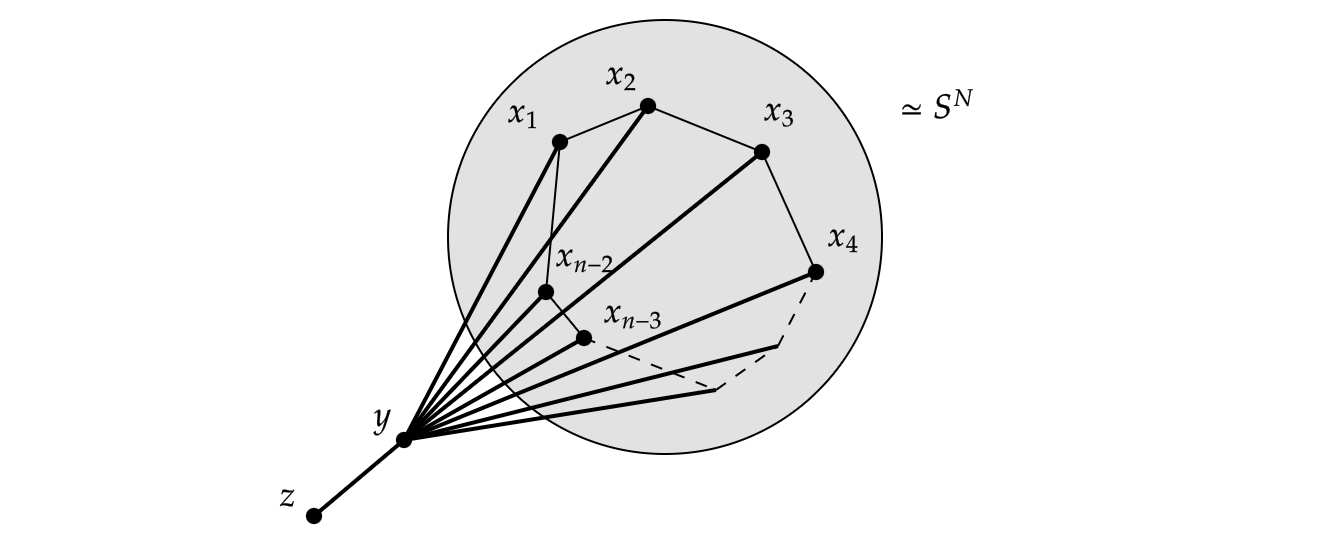
\includegraphics[width=0.8\linewidth]{diagram-20250828.png}
  \end{figure}  

The graph above is that special family of graphs, where $V(G)=\{x_1,x_2,x_3,\cdots,x_{n-3},x_{n-2},y,z\}$ and $\Delta G^c[\{x_1,x_2,x_3,\cdots,x_{n-3},x_{n-2}\}]\simeq S^N$. We let $y$ be adjacent to all the other vertices and $z$ only be adjacent to $y$.

We claim that the $\mathrm{reg}(I_G)=N+2$. Since  $\Delta G^c[\{x_1,x_2,x_3,\cdots,x_{n-3},x_{n-2}\}]\simeq S^N$, by Hochster's formula, $\mathrm{reg}(I_G)\geq N+2$. To show the other direction, we need to analyze the Stanley-Reisner complex of $I_G$. Let $M>N$. As $y$ is adjacent to all the other vertices, it is an isolated vertex in the Stanley-Reisner complex.  Hence, if there is a subcomplex of $\Delta G^c$ whose $M$-dimensional homology is non-trivial, it doesn't need to include $y$, because $y$ can help nothing here. Since $z$ is not adjacent to any $x_i$ in $G$, then the subcomplex on any subset of $\{x_1,x_2,x_3,\cdots,x_{n-3},x_{n-2}\}$ together with $z$ would be a cone, hence contractible. So, if there is a subcomplex of $\Delta G^c$ whose $M$-dimensional homology is non-trivial, it has to be a subcomplex of $\Delta G^c[\{x_1,x_2,x_3,\cdots,x_{n-3},x_{n-2}\}]$. However, this cannot be possible. Consequently, $\mathrm{reg}(I_G)=N+2$.

By the reasoning before, we can also see that, for any subcomplex, if $z$ is in this subcomplex, then this subcomplex would always be contractible unless this subcomplex also involves $y$. Moreover, even we have both $y$ and $z$ simultaneously, we can only get a subcomplex whose $0$-dimensional homology is non-trivial. So, to some sense, the vertex $z$ is the least possible vertex that can contribute to the regularity. If we add $N$ degrees only to vertex $z$, since adding degree is equivalent to adding dimension in homology in this case, we will shift the homology dimension by adding $N$, therefore, any subcomplex involving $y$ and $z$ would be same as $\Delta G^c[\{x_1,x_2,x_3,\cdots,x_{n-3},x_{n-2}\}]$ homologically. So, no subcomplex breaks the homology red line $N$, then the regularity will remain the same.
\end{proof}

%\subsection{A general formula}
%In section 3, we introduced several different types of graphs and the regualrity offset of them. We gave each type of graphs a formula describing the regularity offset which is always in the form of taking the minimum among plenty of things. So, a natural question would be can we establish such kind of formula for all the graphs?







\newpage
\bibliographystyle{plain}
\bibliography{reference}
\end{document}
